%\documentclass[twocolumn,showpacs,prb,superscriptaddress,aps,floatfix]{revtex4-1}
\documentclass[preprint,showpacs,prb,superscriptaddress,aps,floatfix]{revtex4-1}
\usepackage{rotating}
\usepackage{amsmath}
\usepackage{color}
\usepackage{graphicx}
\usepackage{epsfig}
\usepackage{courier}
\usepackage[active]{srcltx}
\usepackage[sort&compress]{natbib}


\newcommand{\uu}{{\bf u}}
\newcommand{\qq}{{\bf q}}
\newcommand{\ab}{{\bf a}}
\newcommand{\bb}{{\bf b}}
\newcommand{\hh}{{\bf h}}
\newcommand{\rr}{{\bf r}}
\newcommand{\pp}{{\bf p}}
\newcommand{\PP}{{\bf P}}
\newcommand{\kk}{{\bf k}}
\newcommand{\HH}{{\bf H}}
\newcommand{\GG}{{\bf G}}
\newcommand{\SiS}{{\bf \Sigma}}
\newcommand{\VV}{{\bf V}}
\newcommand{\UU}{{\bf U}}
\newcommand{\w}{\omega}
\newcommand{\tf}{\textbf}
\newcommand{\bo}{\mathbf}
\newcommand{\br}{{\bf r}}
\newcommand{\be}{\begin{equation}}
\newcommand{\ee}{\end{equation}}
\newcommand{\ben}{\begin{equation*}}
\newcommand{\een}{\end{equation*}}
\newcommand{\bea}{\begin{eqnarray}}
\newcommand{\eea}{\end{eqnarray}}
\newcommand{\bean}{\begin{eqnarray*}}
\newcommand{\eean}{\end{eqnarray*}}
\newcommand{\nup}{n_{\uparrow}}
\newcommand{\ndown}{n_{\downarrow}}
\newcommand{\Id}[1] {\int \! \! {\rm d}^3 #1}
\renewcommand{\v}[1]{{\bf #1}}
\renewcommand{\[}{\left[}
\renewcommand{\]}{\right]}
\renewcommand{\(}{\left(}
\renewcommand{\)}{\right)}
\def\efield{\boldsymbol{\cal E}} 
\def\ket#1{\vert#1\rangle}
\def\bra#1{\langle#1\vert}
\def\pw{^{({\rm W})}}
\def\ph{^{({\rm H})}}
\def\D{{D}\ph}




 
\newcommand{\grenoble}{Institut N\'eel,
CNRS/UJF, 25 rue des Martyrs BP 166, B\^{a}timent D 38042 Grenoble
cedex 9 France} 
\newcommand{\rome}{Istituto di Struttura della Materia (ISM), Consiglio Nazionale delle Ricerche, Via Salaria Km 29.5, CP 10, 00016 Monterotondo Stazione, Italy}
\newcommand{\coimbra}{Centre for Computational Physics and Physics Department, University of Coimbra, Rua Larga, 3004-516 Coimbra, Portugal}

\begin{document}
\title{Simple model for high-harmonic generation}
\author{C. Attaccalite}
\affiliation{\grenoble}

\begin{abstract}
In these notes I consider a simple tight-binding model in Wannier guage and write down the equation of motion of the density matrix in such a way to study its non-linear response and in particular the high-harmonic generation. I discuss all steps for the implementation in a computational code. 
\end{abstract}           

\maketitle

\section{Unit cell and atomic positions}
As simple system I consider a two-dimensional hexagonal boron nitride as shown in Fig.~\ref{fig:hbn_lattice}. 
\begin{figure}
  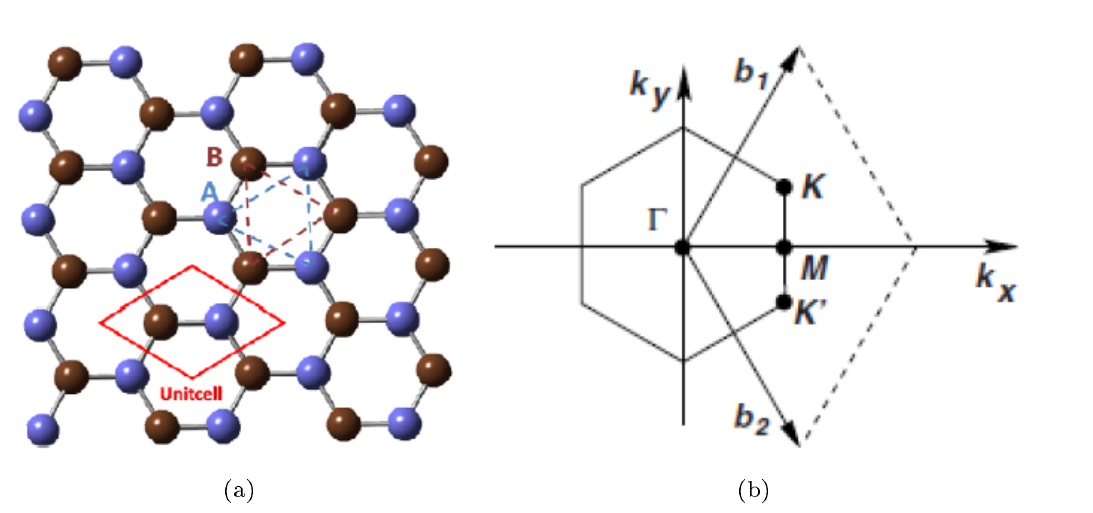
\includegraphics[width=\linewidth]{hbn.png}
  \caption{Hexagonal BN direct and reciprocal lattice.}
  \label{fig:hbn_lattice}
\end{figure}
Lattice vectors are defined as\footnote{I always define quantities in 3D for pratical implementation in the code}:
\bea
a_1&=&\frac{a}{2}\left ( 3, \sqrt{3}, 0 \right)  \\
a_2&=&\frac{a}{2}\left ( 3, -\sqrt{3}, 0 \right)  \\
a_3&=& \left( 0, 0, 1 \right)  \\
\eea
and the volume is $V=a_3 \cdot (a_1 \times a_2) = 3\sqrt{3} a^2/2$ 
and reciprocal lattice vectores are defined as:
\bea
b_1&=&\frac{2\pi}{V} a_2 \times a_3 = \frac{2\pi}{a} \left( 1,  \sqrt{3}, 0\right) \\
b_2&=&\frac{2\pi}{V} a_3 \times a_1 = \frac{2\pi}{a} \left( 1, -\sqrt{3}, 0\right) \\
b_3&=&\frac{2\pi}{V} a_2 \times a_3 = 2\pi \left( 0, 0, 1\right) \\
\eea

\section{Tight binding model}
As simple model consider a two-band tight-binding model with only the first neigboar hopping, and parameters $t_0=2.92~eV$ and $\epsilon_B = -\epsilon_N = 2.81~eV$. The Hamiltonian reads:
\bea
H_{11}(\kk)&=&\epsilon_B\\
H_{22}(\kk)&=&\epsilon_N\\
H_{21}(\kk)&=&H^*_{12}(\kk) = t_0 \cdot e^{-i \kk_y a}\cdot \left(1+2 \cdot e^{i \kk_y \frac{3 a}{2}} \right)\cdot \cos{ \left( \frac{\sqrt{3} a}{2}\kk_x \right) }
\eea 
\section{Wannier and Hamiltonian gauge}
The tight-binding Hamiltonian $H(\kk)$ is a analitic and continous function of $\kk$, therefore I can define all the derivatives respect to $\kk$ without problems. When we diagonalize $H(\kk)$ on a discrete k-point grid, there is a generic phase attached to the eigenvectors that make complicated the derivative respect to $\kk$. We call Wannier gauge the space before the diagonalization  $H^{W}(\kk)$ and Hamiltonian gauge the space after the diagonalization $H^{H}(\kk)$. Wave-function in the two gauges are related by an unitary transformation:
\begin{equation}
\ket{\psi_{n\boldsymbol{k}}^{\left(H\right)}}=\sum_{m}U_{mn}\left(\boldsymbol{k}\right)\ket{\psi_{m\boldsymbol{k}}^{\left(W\right)}}
\end{equation}
where $U\text{\ensuremath{\left(\boldsymbol{k}\right)}}$ is a unitary
matrix that diagonalizes $H^{(W)}\left(\boldsymbol{k}\right)$,
\begin{equation}
U^{\dagger}\text{\ensuremath{\left(\boldsymbol{k}\right)}}H^{(W)}\left(\boldsymbol{k}\right)U\text{\ensuremath{\left(\boldsymbol{k}\right)}}=H^{(H)}\left(\boldsymbol{k}\right).
\end{equation}
Operators that transfor as the Hamiltonian are called gauge covariant. Operator that contains k-derivative are not gauge covariant and require a more complex transformation.\\
Infact consider the transformation:
\begin{equation}
\ket{u_{n\boldsymbol{k}}^{\left(H\right)}}=\sum_{m}U_{mn}\left(\boldsymbol{k}\right)\ket{u_{m\boldsymbol{k}}^{\left(W\right)}}
	\label{u_transf}
\end{equation}
if we derive respect to $\kk$ we get:
\begin{equation}
	\ket{ \partial_{\kk} u_{n\boldsymbol{k}}^{\left(H\right)}}=\sum_{m}U_{mn}\left(\boldsymbol{k}\right)\ket{\partial_{\kk} u_{m\boldsymbol{k}}^{\left(W\right)}} + \sum_{m}\ket{u_{m\boldsymbol{k}}^{\left(W\right)}} \partial_\kk U_{mn}\left(\boldsymbol{k}\right)
	\label{deriv_u}
\end{equation}
the derivative of quantities in Wannier gauges as $\ket{u_{m\boldsymbol{k}}^{\left(W\right)}}$ are not a problem because they are continous functions in $\kk$. We can work out the second term using perturbation theory.\cite{wang2006ab} 
Notice that in the perturbation theory we made a gauge choice, and in particular we choose the "parallel transport" gauge see Sec.~$3.7$ in Ref.~\onlinecite{resta}. \\
We consider an Hamiltonian:
\be
H^{(W)} (\kk + \Delta \kk_\alpha) = H^{(W)} (\kk)  + \Delta \kk_\alpha \partial_\alpha  H^{(W)} (\kk)
\ee
where $\partial_\alpha = \partial/\partial_{\kk_\alpha}$. We consider the second term as a perturbation and write the perturbation theory in the Hamiltonian gauge.
\be
	\ket{ u_{n,\boldsymbol{k}+\Delta \kk}^{\left(H\right)}}=\ket{ u_{n,\boldsymbol{k}}^{\left(H\right)}}+\Delta \kk_\alpha \sum_{m} \frac{\bra{u_{m,\boldsymbol{k} }} H^{(W)}_\alpha   \ket{u_{n,\boldsymbol{k} }}}{\epsilon_{m\kk}-\epsilon_{n\kk}} \ket{u_{m,\boldsymbol{k} }}
\ee
where $ H^{(W)}_\alpha =\partial_\alpha  H^{(W)}$. Then we can define the derivative respect to $\kk$ of an eigenvector as:
\be
\ket{ \partial_\alpha u_{n,\boldsymbol{k}}^{\left(H\right)}}=	\frac{\ket{ u_{n,\boldsymbol{k}+\Delta \kk}^{\left(H\right)}}-\ket{ u_{n,\boldsymbol{k}}^{\left(H\right)}}}{\Delta \kk}= \sum_{m} \frac{\bra{u_{m,\boldsymbol{k} }} H^{(W)}_\alpha   \ket{u_{n,\boldsymbol{k} }}}{\epsilon^{(H)}_{m\kk}-\epsilon(H)_{n\kk}} \ket{u_{m,\boldsymbol{k} }}
\ee
in matrix notation it becomes $ \partial_\alpha U_{mn} = \sum_l U_{ml} D^{(H)}_{ln\alpha}$ and
\begin{equation}
\D_{nm,\alpha}\equiv (U^{\dagger}
\partial_{\alpha}U)_{nm}=
\begin{cases}
  \displaystyle
  \frac{\overline H_{nm,\alpha}^{(\rm H)}}{{\cal E}^{(\rm H)}_{m}
  -{\cal E}_{n}^{(\rm H)}}& \text{if $n\not= m$}\\ \\
  0& \text{if $n=m$}
\end{cases}
\label{eq:ddef}
\end{equation}
If we insert this result in Eq.~\ref{deriv_u} and together with Eq.~\ref{u_transf} we get:
\begin{equation}
	\ket{ \partial_{\kk} u_{n\boldsymbol{k}}^{\left(H\right)}}=\sum_{m}U_{mn}\left(\boldsymbol{k}\right)\ket{\partial_{\kk} u_{m\boldsymbol{k}}^{\left(W\right)}} + \sum_{m}\ket{u_{m\boldsymbol{k}}\ph} \D_{mn,\alpha}
	\label{deriv_uh}
\end{equation}
we will use this result to define the position operator.

\section{Position operator in periodic system}
The position operator in periodic system is defined as:\cite{blount1962solid}
\be
\hat \rr = i \frac{\partial}{\partial \kk} + \hat A
\ee
where $\hat A$ is the transition dipole moment or a generalization of the Berry connection:\cite{silva2019high,wang2006ab}
\be
\boldsymbol{A}\pw_{nm}\left(\boldsymbol{k}\right)=i\int_{V_{C}}d^{D}\boldsymbol{r}\left(u_{n\boldsymbol{k}}\left(\boldsymbol{r}\right)\right)^{*}\frac{\partial}{\partial\boldsymbol{k}}u_{m\boldsymbol{k}}\left(\boldsymbol{r}\right).
\ee
using Eq.~\ref{deriv_uh} this term can be rewritten the Hamiltonian gauge as:
\begin{equation}
\boldsymbol{A}^{\left(H\right)}\left(\boldsymbol{k}\right)=U^{\dagger}\text{\ensuremath{\left(\boldsymbol{k}\right)}}\boldsymbol{A}^{\left(W\right)}\left(\boldsymbol{k}\right)U\text{\ensuremath{\left(\boldsymbol{k}\right)}}+iU^{\dagger}\text{\ensuremath{\left(\boldsymbol{k}\right)}}\frac{\partial}{\partial\boldsymbol{k}}U\left(\boldsymbol{k}\right).
\end{equation}
The term $(U^{\dagger}\partial_{\alpha}U)_{nm}$ can be calculated using perturbation theory as deriving directly the eigenvectors if the phase has been fixed. For example in Ref.~\onlinecite{silva2019high} they fix the phase of the eigenvectors by rotating U such that the diagonal of U is real and positive. Notice the this procedure works only if you do not have degenerate states as in their work.\\
The other therm $\boldsymbol{A}^{\left(W\right)}$ can be calculated in different ways: 
\begin{itemize}
\item
Using matrix elements of the position operator in a Wannier basis:
\be
\boldsymbol{A}_{nm}^{(W)}\left(\boldsymbol{k}\right)  \equiv\sum_{\boldsymbol{R}}e^{i\boldsymbol{k}.\boldsymbol{R}}\left\langle \boldsymbol{0}n\left|\hat{\boldsymbol{r}}\right|\boldsymbol{R}m\right\rangle .\label{eq:Berry_connection_Wannier}
\ee
\item In tight-binding using the approximation:\cite{silva2019high}
\be
		\left\langle \boldsymbol{0}n\left|\hat{\boldsymbol{r}}\right|\boldsymbol{R}m\right\rangle=\delta_{nm}\delta_{\boldsymbol{0} \boldsymbol{R}} = \tau_n
\ee
where $\tau_n$ is the center of the n-Wannier function.
\item 
	From the overlaps of the eigenfunctions:\cite{wang2006ab}
	\begin{equation}
        A_{nm,\alpha}\pw(\kk)\simeq
        i\sum_\bb\,
        w_b b_{\alpha}\Big ( \langle u_{n\kk}\pw|u_{m,\kk+\bb}\pw
        \rangle
        - \delta_{nm}\Big )\;,
\label{eq:A_dis}
\end{equation}
%
where $\bb$ are the vectors connecting $\kk$ to its nearest
neighbors on the {\it ab-initio} mesh, and $w_b$ are the coefficent for the finite difference derivatives. \\
Finally the term  $i {\partial}/{\partial \kk}$ can be calculated directly as a finite difference k-point mesh of the density matrix in the Wannier guage.
\end{itemize}
\appendix
\section{Derivatives in k-space}
In general to perform derivative in k-space we define quantities as:
\be
\PP = \frac{1}{2\pi} \sum_{i=1,3} \ab_i (\PP \cdot \bb_i) = \frac{1}{2\pi} \sum_{i=1,3} \ab_i \PP_i
\ee
where $\bb_i$ are reciprocal lattice vectors and $\ab_i$ direct lattice vectors that satisfy the relation:
\be
\ab_i \cdot \bb_j = 2\pi\delta_{ij}
\ee
then the derivative along a $\bb_i$ vector can be rewritten in cartesian coordinates as:
\be
\nabla \PP = \frac{1}{2\pi} \sum_{i=1,3} \ab_i \left( \frac{\partial \PP_i}{\partial \kk_i} |\bb_i| \right)
\ee 
where $\partial \PP_i/\partial \kk_i$ is the derivative along the $\bb_i$ direction, or one can write the finite difference derivative using $\Delta \kk_i = \bb_i/N_i$.
\be
\nabla \PP = \frac{1}{2\pi} \sum_{i=1,3} \ab_i \left( \frac{\Delta \PP_i}{\Delta \kk_i}  |\bb_i|  \right) = \frac{1}{2\pi} \sum_{i=1,3} \ab_i \left( N_i \Delta \PP_i \right)
\ee 

\addcontentsline{toc}{chapter}{Bibliography}
\bibliographystyle{apsrev4-1}
\bibliography{hhg}
\end{document}
